\documentclass[10pt,aspectratio=169]{beamer}

\usepackage[T1]{fontenc}
\usepackage[utf8]{inputenc}
\usepackage{lmodern}
\usepackage{amsmath,amssymb}
\usepackage{booktabs,array,tabularx}
\usepackage{graphicx}
\usepackage{tikz}
\usetikzlibrary{arrows.meta,calc,fit,positioning,shapes.geometric}

% -----------------------------------------------------------------------------
% Visual identity
% -----------------------------------------------------------------------------
\definecolor{DeepNavy}{HTML}{17324D}
\definecolor{BrazilGreen}{HTML}{1B7F5A}
\definecolor{WarmGold}{HTML}{E3A72F}
\definecolor{Brick}{HTML}{B84A4A}
\definecolor{Sky}{HTML}{EAF2F6}
\definecolor{WarmGray}{HTML}{F4F2EE}
\definecolor{MidGray}{HTML}{66717A}
\definecolor{DarkText}{HTML}{17212B}

\setbeamercolor{normal text}{fg=DarkText,bg=white}
\setbeamercolor{structure}{fg=BrazilGreen}
\setbeamercolor{frametitle}{fg=DeepNavy,bg=white}
\setbeamercolor{title}{fg=white}
\setbeamercolor{subtitle}{fg=Sky}
\setbeamercolor{alerted text}{fg=Brick}
\setbeamercolor{block title}{fg=white,bg=DeepNavy}
\setbeamercolor{block body}{fg=DarkText,bg=Sky}
\setbeamercolor{exampleblock title}{fg=white,bg=BrazilGreen}
\setbeamercolor{exampleblock body}{fg=DarkText,bg=WarmGray}

\setbeamerfont{title}{size=\LARGE,series=\bfseries}
\setbeamerfont{subtitle}{size=\large}
\setbeamerfont{frametitle}{size=\Large,series=\bfseries}
\setbeamerfont{footline}{size=\scriptsize}
\setbeamerfont{block title}{series=\bfseries}

\setbeamertemplate{navigation symbols}{}
\setbeamertemplate{itemize item}{\color{BrazilGreen}$\blacktriangleright$}
\setbeamertemplate{itemize subitem}{\color{WarmGold}$\bullet$}
\setbeamertemplate{frametitle}{%
  \vspace{0.15cm}\insertframetitle\par
  \vspace{0.05cm}\color{BrazilGreen}\rule{\textwidth}{0.7pt}}
\setbeamertemplate{footline}{%
  \leavevmode%
  \hbox{%
    \begin{beamercolorbox}[wd=.78\paperwidth,ht=2.5ex,dp=1.1ex,leftskip=.45cm]{author in head/foot}%
      \color{MidGray}The Brazilian Agenda of Economic Development
    \end{beamercolorbox}%
    \begin{beamercolorbox}[wd=.22\paperwidth,ht=2.5ex,dp=1.1ex,rightskip=.45cm plus1fil]{date in head/foot}%
      \hfill\color{MidGray}\insertframenumber/\inserttotalframenumber
    \end{beamercolorbox}}}

\hypersetup{colorlinks=true,urlcolor=BrazilGreen,linkcolor=DeepNavy}
\renewcommand{\arraystretch}{1.25}
\graphicspath{{brazilian_development_agenda_assets/}}

\newcommand{\source}[1]{%
  \par\vfill{\tiny\color{MidGray}Source: #1}}
\newcommand{\key}[1]{\textcolor{BrazilGreen}{\textbf{#1}}}
\newcommand{\warn}[1]{\textcolor{Brick}{\textbf{#1}}}
\newcommand{\muted}[1]{\textcolor{MidGray}{#1}}
\newcommand{\datagraphic}[1]{%
  \begin{center}\includegraphics[width=.94\textwidth,height=.50\textheight,keepaspectratio]{#1}\end{center}}
\newcommand{\question}[1]{%
  \begin{beamercolorbox}[rounded=true,sep=0.55em,wd=\textwidth]{block body}
    \centering\large\textbf{#1}
  \end{beamercolorbox}}
\newcommand{\sectionframe}[2]{%
  \begin{frame}[plain]
    \begin{tikzpicture}[remember picture,overlay]
      \fill[DeepNavy] (current page.south west) rectangle (current page.north east);
      \fill[BrazilGreen] (current page.south west) rectangle
        ([xshift=0.23\paperwidth]current page.north west);
      \node[anchor=west,text=white,font=\bfseries\fontsize{25}{28}\selectfont,
            text width=.66\paperwidth]
        at ([xshift=.29\paperwidth,yshift=.05\paperheight]current page.west) {#1};
      \node[anchor=west,text=Sky,font=\large,text width=.62\paperwidth]
        at ([xshift=.29\paperwidth,yshift=-.10\paperheight]current page.west) {#2};
    \end{tikzpicture}
  \end{frame}}

\title{The Brazilian Agenda of\\Economic Development}
\subtitle{Macroeconomic stability, productivity, state capacity, and inclusion}
\author{Eduardo Peres Cunha}
\institute{PUC-Rio -- Brazilian Seminars}
\date{July 2026}

\begin{document}

% 01
\begin{frame}[plain]
  \begin{tikzpicture}[remember picture,overlay]
    \fill[DeepNavy] (current page.south west) rectangle (current page.north east);
    \fill[BrazilGreen] (current page.south west) rectangle
      ([xshift=.18\paperwidth]current page.north west);
    \fill[WarmGold] ([xshift=.18\paperwidth]current page.south west) rectangle
      ([xshift=.195\paperwidth]current page.north west);
    \node[anchor=west,text=white,text width=.72\paperwidth]
      at ([xshift=.25\paperwidth,yshift=.12\paperheight]current page.west)
      {\usebeamerfont{title}\inserttitle};
    \node[anchor=west,text=Sky,text width=.65\paperwidth]
      at ([xshift=.25\paperwidth,yshift=-.03\paperheight]current page.west)
      {\usebeamerfont{subtitle}\insertsubtitle};
    \node[anchor=west,text=white,font=\normalsize]
      at ([xshift=.25\paperwidth,yshift=-.22\paperheight]current page.west)
      {\insertauthor\quad | \quad\insertinstitute\quad | \quad\insertdate};
  \end{tikzpicture}
\end{frame}
% Olá Eduardo
% 02
\begin{frame}{The lecture starts from one puzzle}
  \vspace{0.7cm}
  \question{Why has a large, urban, resource-rich economy with strong institutions in selected areas failed to achieve sustained income convergence?}
  \vspace{0.8cm}
  \begin{columns}[T,onlytextwidth]
    \column{.31\textwidth}
      \begin{block}{Past achievement}
        Rapid industrialization and urbanization.
      \end{block}
    \column{.31\textwidth}
      \begin{block}{Institutional achievement}
        Stabilization, social policy, agriculture, and digital payments.
      \end{block}
    \column{.31\textwidth}
      \begin{block}{Unfinished transition}
        Low aggregate productivity and persistent inequality.
      \end{block}
  \end{columns}
\end{frame}

% 03
\begin{frame}{Brazil combines frontier capabilities with large deficits}
  \begin{columns}[T,onlytextwidth]
    \column{.49\textwidth}
      \begin{beamercolorbox}[rounded=true,sep=.7em,wd=\textwidth]{block body}
        \key{Continental scale}\par
        More than 200 million people and 5,500 municipalities.
      \end{beamercolorbox}
      \vspace{.35cm}
      \begin{beamercolorbox}[rounded=true,sep=.7em,wd=\textwidth]{exampleblock body}
        \key{Clean electricity}\par
        86.6\% of domestic electricity supply was renewable in 2025.
      \end{beamercolorbox}
    \column{.49\textwidth}
      \begin{beamercolorbox}[rounded=true,sep=.7em,wd=\textwidth]{exampleblock body}
        \key{Institutional innovation}\par
        Pix scaled digital public infrastructure to most adults.
      \end{beamercolorbox}
      \vspace{.35cm}
      \begin{beamercolorbox}[rounded=true,sep=.7em,wd=\textwidth]{block body}
        \warn{Persistent duality}\par
        38.1\% of workers remained informal in 2025.
      \end{beamercolorbox}
  \end{columns}
  \source{World Bank, Brazil Overview; EPE, BEN 2026; BCB, Pix statistics; IBGE, PNAD Continua 2025.}
\end{frame}

% 05
\begin{frame}{Development is broader than current GDP growth}
  \begin{columns}[T,onlytextwidth]
    \column{.24\textwidth}\begin{block}{Income}\centering Income per person\end{block}
    \column{.24\textwidth}\begin{block}{Productivity}\centering Output per worker\end{block}
    \column{.24\textwidth}\begin{block}{Inclusion}\centering Mobility and access\end{block}
    \column{.24\textwidth}\begin{block}{Resilience}\centering Climate and institutions\end{block}
  \end{columns}
  \vspace{.35cm}
  \[
    \frac{Y}{N}=\underbrace{\frac{Y}{L}}_{\text{output per worker}}
    \times
    \underbrace{\frac{L}{N}}_{\text{workers per person}}
  \]
  \begin{itemize}
    \item Productivity determines how much each worker produces.
    \item Demography and labor-force participation determine how many people work.
    \item Distribution determines who can invest in skills and participate.
  \end{itemize}
\end{frame}

% 06
\begin{frame}{Roadmap for 150 minutes}
  \small
  \begin{tabularx}{\textwidth}{>{\bfseries}p{1.8cm}p{3.3cm}X}
    \toprule
    Time & Block & Main question \\
    \midrule
    0--12 min & The puzzle & What counts as development? \\
    12--65 min & Macro foundations & How do inflation, fiscal policy, and exchange rates shape growth? \\
    65--75 min & Exchange-rate case & What changed in 1999, and why does the regime matter? \\
    75--85 min & Break &  \\
    85--135 min & Micro constraints & Firms, workers, infrastructure, security, and state capacity \\
    135--147 min & Integrated agenda & Which reforms are complements? \\
    147--150 min & Questions & Which constraint changes the rest of the agenda? \\
    \bottomrule
  \end{tabularx}
\end{frame}

% 07
\sectionframe{Part I -- Making growth possible}{Macroeconomic stability, exchange-rate regimes, fiscal space, and investment}

\begin{frame}{Growth has been volatile and convergence has been intermittent}
  \datagraphic{fig_real_gdp_growth.pdf}
  \begin{itemize}
    \item Brazil combined strong expansions with three recessions after 1995.
    \item The post-2010 problem is not one crisis alone: average growth weakened before the pandemic.
  \end{itemize}
  \source{BCB SGS 7326, based on IBGE National Accounts. Annual real GDP growth; 2025 is the latest observation.}
\end{frame}

% 08
\begin{frame}{High inflation disrupts more than purchasing power}
  \datagraphic{fig_ipca_12m.pdf}
  \begin{itemize}
    \item Stabilization restored price information and lengthened planning horizons.
    \item The later spikes show why credibility, fiscal policy, and the exchange rate still interact.
  \end{itemize}
  \source{BCB SGS 433, monthly IPCA. Twelve-month rates are compounded from the official monthly series.}
\end{frame}

% 09
\begin{frame}{The Real Plan changed the unit of account before the currency}
  \begin{center}
  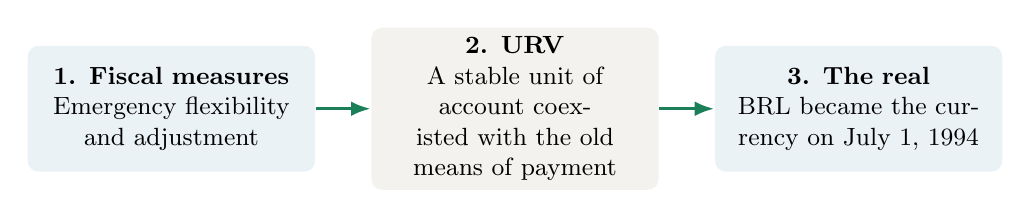
\begin{tikzpicture}[node distance=.7cm,
    stage/.style={rounded corners,minimum width=3.65cm,minimum height=1.6cm,
                  align=center,text width=3.4cm,font=\small,draw=none}]
    \node[stage,fill=Sky] (fiscal) {\textbf{1. Fiscal measures}\\Emergency flexibility and adjustment};
    \node[stage,fill=WarmGray,right=of fiscal] (urv) {\textbf{2. URV}\\A stable unit of account coexisted with the old means of payment};
    \node[stage,fill=Sky,right=of urv] (real) {\textbf{3. The real}\\BRL became the currency on July 1, 1994};
    \draw[-{Latex[length=2.5mm]},very thick,BrazilGreen] (fiscal) -- (urv);
    \draw[-{Latex[length=2.5mm]},very thick,BrazilGreen] (urv) -- (real);
  \end{tikzpicture}
  \end{center}
  \vspace{.6cm}
  \begin{itemize}
    \item The URV coordinated prices without an overnight freeze.
    \item Its value was linked to the U.S. dollar during the transition.
    \item The exchange rate then became part of the nominal anchor.
  \end{itemize}
  \source{BCB, \href{https://www.bcb.gov.br/en/monetarypolicy/realplan}{The Real Plan}.}
\end{frame}

\begin{frame}{The Real Plan produced a discrete break in inflation}
  \datagraphic{fig_ipca_pre_post_real.pdf}
  \begin{itemize}
    \item Twelve-month inflation reached thousands of percent before July 1994.
    \item From July 1995 onward, every month in the twelve-month window uses prices quoted under the Real.
  \end{itemize}
  \source{BCB SGS 433, monthly IPCA. Rates are compounded over twelve months. The two panels use different vertical scales.}
\end{frame}

% 10
\begin{frame}{The exchange rate links the macroeconomy to development}
  \begin{center}
  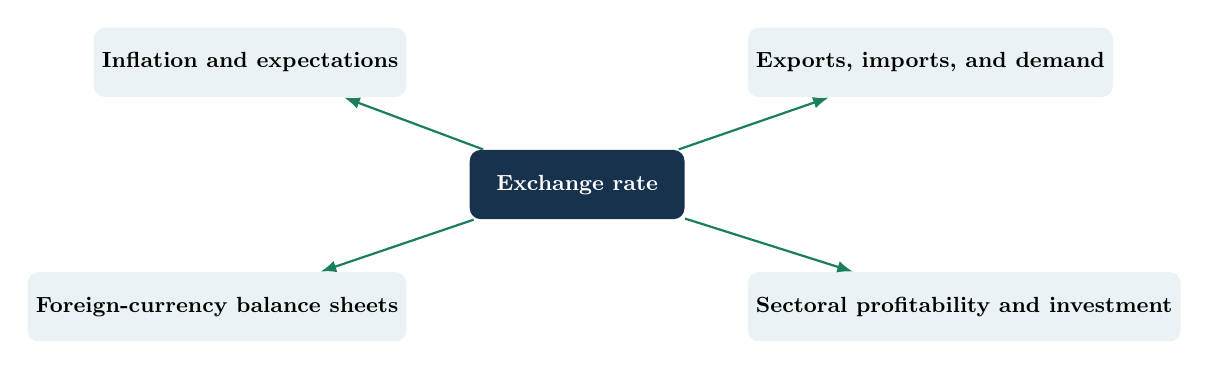
\begin{tikzpicture}[scale=.88,every node/.style={transform shape},node distance=.75cm and .9cm,
    box/.style={rounded corners,fill=Sky,minimum width=3.1cm,minimum height=1.0cm,
                align=center,font=\small\bfseries},
    arr/.style={-{Latex[length=2mm]},thick,BrazilGreen}]
    \node[box,fill=DeepNavy,text=white] (fx) {Exchange rate};
    \node[box,above left=of fx] (prices) {Inflation and expectations};
    \node[box,above right=of fx] (trade) {Exports, imports, and demand};
    \node[box,below left=of fx] (finance) {Foreign-currency balance sheets};
    \node[box,below right=of fx] (structure) {Sectoral profitability and investment};
    \draw[arr] (fx) -- (prices);
    \draw[arr] (fx) -- (trade);
    \draw[arr] (fx) -- (finance);
    \draw[arr] (fx) -- (structure);
  \end{tikzpicture}
  \end{center}
  \vspace{.35cm}
  \question{An exchange-rate regime allocates adjustment across the currency, interest rates, reserves, and domestic demand.}
\end{frame}

% 11
\begin{frame}{Brazil moved from managed adjustment to a formal float}
  \centering
  \resizebox{.96\textwidth}{!}{%
  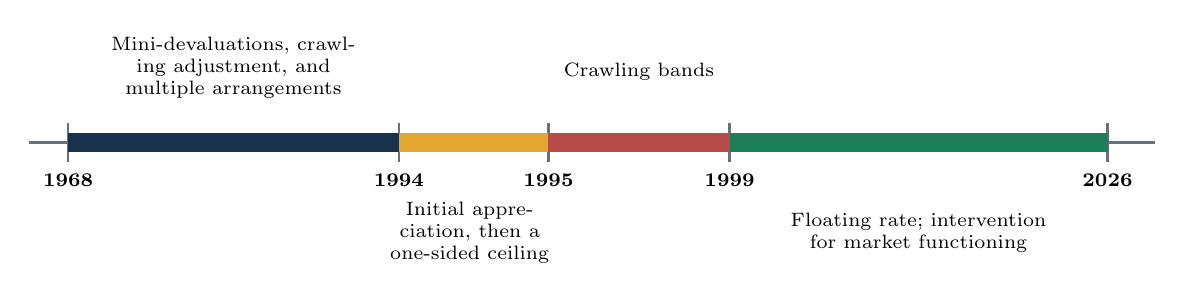
\begin{tikzpicture}[x=1cm,y=1cm]
    \draw[thick,MidGray] (.5,2.4) -- (14.8,2.4);
    \foreach \x/\yr in {1/1968,5.2/1994,7.1/1995,9.4/1999,14.2/2026}{
      \draw[thick,MidGray] (\x,2.15) -- (\x,2.65);
      \node[font=\scriptsize\bfseries,below] at (\x,2.12) {\yr};}
    \draw[line width=7pt,DeepNavy] (1,2.4) -- (5.2,2.4);
    \draw[line width=7pt,WarmGold] (5.2,2.4) -- (7.1,2.4);
    \draw[line width=7pt,Brick] (7.1,2.4) -- (9.4,2.4);
    \draw[line width=7pt,BrazilGreen] (9.4,2.4) -- (14.2,2.4);
    \node[align=center,font=\scriptsize,text width=3.5cm] at (3.1,3.35)
      {Mini-devaluations, crawling adjustment, and multiple arrangements};
    \node[align=center,font=\scriptsize,text width=2.1cm] at (6.1,1.25)
      {Initial appreciation, then a one-sided ceiling};
    \node[align=center,font=\scriptsize,text width=2.5cm] at (8.25,3.3)
      {Crawling bands};
    \node[align=center,font=\scriptsize,text width=4.0cm] at (11.8,1.25)
      {Floating rate; intervention for market functioning};
  \end{tikzpicture}
  }
  \vspace{.25cm}
  \begin{minipage}{.96\textwidth}
  \begin{itemize}
    \item Historical labels summarize changing rules and multiple market segments.
    \item The operational regime can differ from a simple fixed-versus-floating label.
  \end{itemize}
  \end{minipage}
  \source{BCB, 1999 FX Market Analysis and official FX-policy pages; dates before 1994 are a schematic summary.}
\end{frame}

\begin{frame}{The exchange rate adjusted after the 1999 regime change}
  \datagraphic{fig_brl_usd.pdf}
  \begin{itemize}
    \item The band limited adjustment before 1999; the float then absorbed domestic and external shocks.
    \item A weaker real is not a development policy by itself: relative prices, balance sheets, and persistence matter.
  \end{itemize}
  \source{BCB SGS 3692. BRL per US dollar, selling rate at year-end; shaded period marks the explicit-band era.}
\end{frame}

% 12
\begin{frame}{The policy trilemma makes the trade-off explicit}
  \begin{columns}[T,onlytextwidth]
    \column{.43\textwidth}
      \begin{center}
      \resizebox{.92\linewidth}{!}{%
      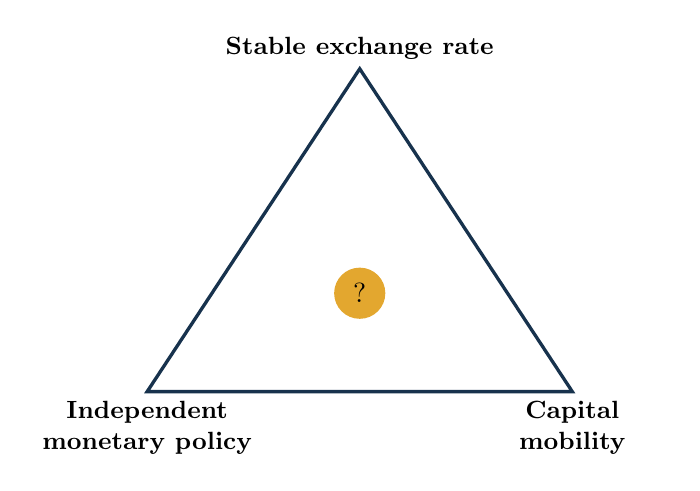
\begin{tikzpicture}
        \coordinate (A) at (0,3.5);
        \coordinate (B) at (-2.7,-.6);
        \coordinate (C) at (2.7,-.6);
        \draw[very thick,DeepNavy] (A)--(B)--(C)--cycle;
        \node[above,align=center,font=\small\bfseries] at (A) {Stable exchange rate};
        \node[below,align=center,font=\small\bfseries,text width=2.8cm] at (B) {Independent monetary policy};
        \node[below,align=center,font=\small\bfseries,text width=2.3cm] at (C) {Capital mobility};
        \node[circle,fill=WarmGold,minimum size=.65cm] at (0,.65) {?};
      \end{tikzpicture}
      }
      \end{center}
    \column{.54\textwidth}
      \begin{itemize}
        \item A country can fully pursue only two corners at once.
        \item Under an exchange-rate anchor, interest rates defend the parity.
        \item Under a float, the currency absorbs part of external shocks.
        \item Capital-flow measures change the constraint but do not remove it.
      \end{itemize}
  \end{columns}
\end{frame}

% 13
\begin{frame}{The Real used the exchange rate as a nominal anchor}
  \begin{columns}[T,onlytextwidth]
    \column{.49\textwidth}
      \begin{block}{Why it helped}
        A stable currency price disciplined tradable-goods prices and coordinated expectations after hyperinflation.
      \end{block}
      \vspace{.25cm}
      \begin{exampleblock}{Why pressure accumulated}
        Domestic inflation exceeded foreign inflation, the real appreciated, and high interest rates attracted capital while defending the regime.
      \end{exampleblock}
    \column{.47\textwidth}
      \begin{itemize}
        \item July--September 1994 first allowed the real to appreciate below BRL 1 per USD.
        \item September introduced a one-sided BRL 1 per USD dollar-sale ceiling, not a fixed parity.
        \item Explicit symmetric bands began in March 1995.
        \item The currency depreciated gradually inside a managed corridor.
        \item External shocks tested reserve and interest-rate defenses.
      \end{itemize}
  \end{columns}
  \source{BCB, FX Market Analysis, 1999 Q1.}
\end{frame}

% 14
\begin{frame}{A crawling band trades flexibility for credibility}
  \begin{center}
  \resizebox{.88\textwidth}{!}{%
  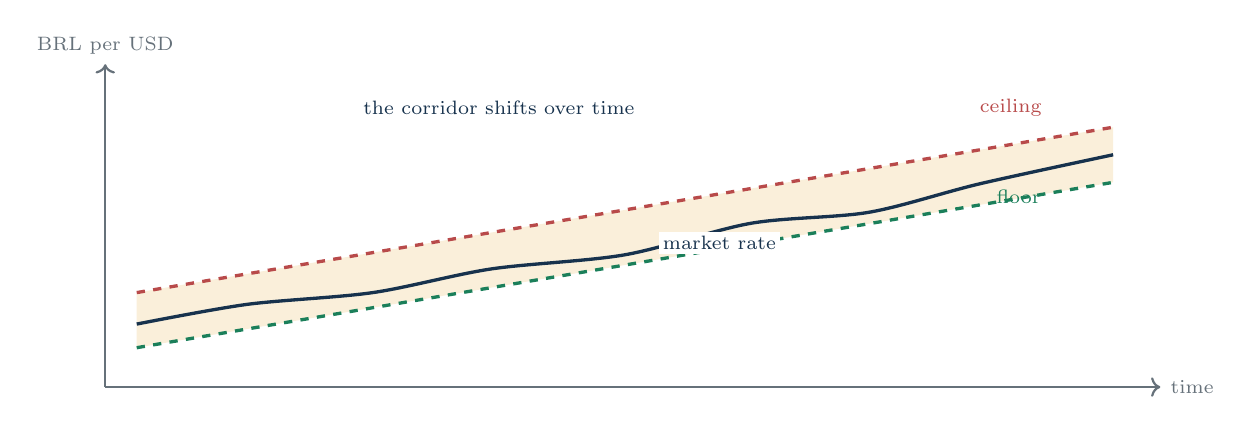
\begin{tikzpicture}[x=1cm,y=1cm]
    \draw[->,thick,MidGray] (.4,.5) -- (13.8,.5) node[right,font=\scriptsize]{time};
    \draw[->,thick,MidGray] (.4,.5) -- (.4,4.6) node[above,font=\scriptsize]{BRL per USD};
    \fill[WarmGold!18] (.8,1.0) -- (13.2,3.1) -- (13.2,3.8) -- (.8,1.7) -- cycle;
    \draw[very thick,Brick,dashed] (.8,1.7) -- (13.2,3.8);
    \draw[very thick,BrazilGreen,dashed] (.8,1.0) -- (13.2,3.1);
    \draw[very thick,DeepNavy] plot[smooth] coordinates
      {(.8,1.3)(2.2,1.55)(3.8,1.7)(5.3,2.0)(7.0,2.18)(8.6,2.58)(10.1,2.72)(11.5,3.08)(13.2,3.45)};
    \node[font=\scriptsize,text=Brick] at (11.9,4.05) {ceiling};
    \node[font=\scriptsize,text=BrazilGreen] at (12.0,2.92) {floor};
    \node[font=\scriptsize,text=DeepNavy,fill=white,inner sep=1.5pt] at (8.2,2.33) {market rate};
    \node[align=center,font=\scriptsize,text=DeepNavy] at (5.4,4.05)
      {the corridor shifts over time};
  \end{tikzpicture}
  }
  \end{center}
  \begin{itemize}
    \item The market rate fluctuates inside the corridor while the authorities move its boundaries over time.
    \item A narrow corridor can strengthen the anchor but invites one-way bets when fundamentals diverge.
  \end{itemize}
  \source{Stylized diagram; BCB, 1999 Q1 FX Market Analysis.}
\end{frame}

% 15
\begin{frame}{January 1999 compressed a regime change into five days}
  \begin{center}
  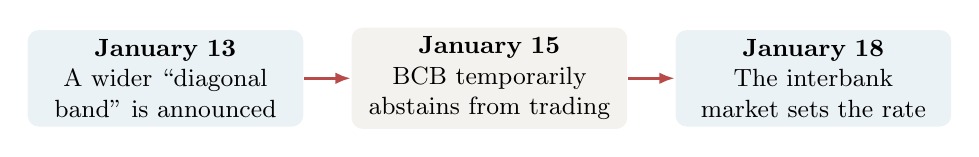
\begin{tikzpicture}[node distance=.6cm,
    date/.style={rounded corners,minimum width=3.5cm,minimum height=1.2cm,
                 text width=3.2cm,align=center,font=\small}]
    \node[date,fill=Sky] (d13) {\textbf{January 13}\\A wider ``diagonal band'' is announced};
    \node[date,fill=WarmGray,right=of d13] (d15) {\textbf{January 15}\\BCB temporarily abstains from trading};
    \node[date,fill=Sky,right=of d15] (d18) {\textbf{January 18}\\The interbank market sets the rate};
    \draw[-{Latex[length=2mm]},very thick,Brick] (d13)--(d15);
    \draw[-{Latex[length=2mm]},very thick,Brick] (d15)--(d18);
  \end{tikzpicture}
  \end{center}
  \vspace{.55cm}
  \begin{itemize}
    \item The BCB retained the option to intervene against disorderly movements.
    \item Formal inflation targeting followed in July 1999.
    \item The nominal anchor shifted from the exchange rate to the inflation target.
  \end{itemize}
  \source{BCB, \href{https://www.bcb.gov.br/estabilidadefinanceira/exibenormativo?numero=6565&tipo=Comunicado}{Communique 6,565}; BCB Working Paper 25.}
\end{frame}

% 16
\begin{frame}{Since 1999, the exchange rate floats and the BCB targets inflation}
  \begin{columns}[T,onlytextwidth]
    \column{.48\textwidth}
      \begin{block}{Formal regime}
        The market determines the exchange rate. The BCB does not intervene to select a level.
      \end{block}
      \vspace{.25cm}
      \begin{block}{Monetary anchor}
        The policy rate responds to the inflation outlook under an explicit target.
      \end{block}
    \column{.48\textwidth}
      \begin{exampleblock}{Adjustment mechanism}
        The currency absorbs part of external shocks while interest rates respond to the inflation outlook.
      \end{exampleblock}
      \vspace{.25cm}
      \question{The nominal anchor moved from the exchange rate to the inflation target.}
  \end{columns}
  \source{BCB, \href{https://www.bcb.gov.br/en/financialstability/fxpolicy}{Foreign Exchange Policy}.}
\end{frame}

\begin{frame}{Monetary policy reacts to the inflation outlook}
  \datagraphic{fig_selic_ipca.pdf}
  \begin{itemize}
    \item The policy rate is forward-looking; it need not move one-for-one with current inflation.
    \item Fiscal risk and exchange-rate pass-through affect how much tightening is required.
  \end{itemize}
  \source{BCB SGS 432 and 433. Selic target is the last observation of each month; IPCA is compounded over 12 months.}
\end{frame}

% 18
\begin{frame}{Nominal and real exchange rates answer different questions}
  \begin{columns}[T,onlytextwidth]
    \column{.46\textwidth}
      \begin{block}{Nominal rate}
        \[
          E=\text{BRL per USD}
        \]
        A rise in $E$ is a nominal depreciation of the real.
      \end{block}
    \column{.50\textwidth}
      \begin{exampleblock}{Real exchange rate}
        \[
          q=\frac{E P^{*}}{P}
        \]
        A rise in $q$ makes foreign goods more expensive relative to domestic goods under this definition.
      \end{exampleblock}
  \end{columns}
  \vspace{.4cm}
  \begin{itemize}
    \item Domestic and foreign inflation can undo a nominal depreciation.
    \item Productivity, terms of trade, and risk premia affect the equilibrium real rate.
    \item ``Competitive'' has no meaning without a price index, horizon, and sector.
  \end{itemize}
\end{frame}

% 19
\begin{frame}{A depreciation reaches inflation through several margins}
  \begin{center}
  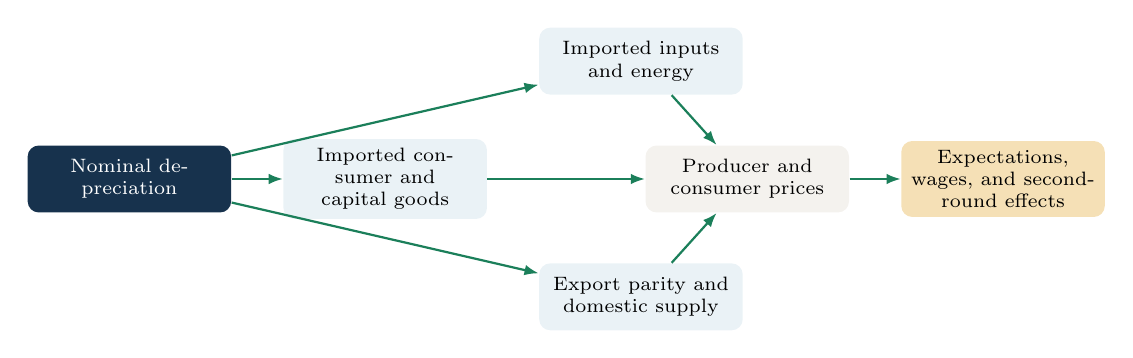
\begin{tikzpicture}[node distance=.55cm and .65cm,
    box/.style={rounded corners,fill=Sky,minimum height=.85cm,text width=2.35cm,
                align=center,font=\scriptsize},
    arr/.style={-{Latex[length=1.8mm]},thick,BrazilGreen}]
    \node[box,fill=DeepNavy,text=white] (dep) {Nominal depreciation};
    \node[box,right=of dep] (imports) {Imported consumer and capital goods};
    \node[box,above right=of imports] (inputs) {Imported inputs and energy};
    \node[box,below right=of imports] (exports) {Export parity and domestic supply};
    \node[box,right=2.0cm of imports,fill=WarmGray] (prices) {Producer and consumer prices};
    \node[box,right=of prices,fill=WarmGold!35] (expect) {Expectations, wages, and second-round effects};
    \draw[arr] (dep)--(imports);
    \draw[arr] (dep)--(inputs);
    \draw[arr] (dep)--(exports);
    \draw[arr] (imports)--(prices);
    \draw[arr] (inputs)--(prices);
    \draw[arr] (exports)--(prices);
    \draw[arr] (prices)--(expect);
  \end{tikzpicture}
  \end{center}
  \vspace{.4cm}
  \question{Pass-through depends on expectations, slack, margins, initial inflation, and the size of the shock.}
  \source{BCB Working Papers 5, 181, and 473.}
\end{frame}

% 20
\begin{frame}{Exchange-rate pass-through is state-dependent}
  \begin{columns}[T,onlytextwidth]
    \column{.49\textwidth}
      \begin{beamercolorbox}[rounded=true,sep=.7em,wd=\textwidth]{exampleblock body}
        \key{Normal conditions}\par
        Credible targets, anchored expectations, slack, and smaller shocks limit propagation.
      \end{beamercolorbox}
    \column{.49\textwidth}
      \begin{beamercolorbox}[rounded=true,sep=.7em,wd=\textwidth]{block body}
        \warn{Crisis conditions}\par
        Large depreciations, high uncertainty, indexation, and unanchored expectations raise propagation.
      \end{beamercolorbox}
  \end{columns}
  \vspace{.75cm}
  \begin{itemize}
    \item A 2026 BCB exercise estimates that a 10\% depreciation adds about 1.0 percentage point to IPCA over 12 months and 1.6 points over 24 months.
    \item The confidence bands are wide, and the effects differ sharply across food, industrial goods, and services.
    \item Monetary policy responds to the inflation forecast, not mechanically to the exchange rate.
  \end{itemize}
  \source{BCB, March 2026 Monetary Policy Report, exchange-rate pass-through box; estimates are episode-dependent.}
\end{frame}

% 21
\begin{frame}{Commodities affect the currency and the production structure}
  \begin{center}
  \resizebox{.92\textwidth}{!}{%
  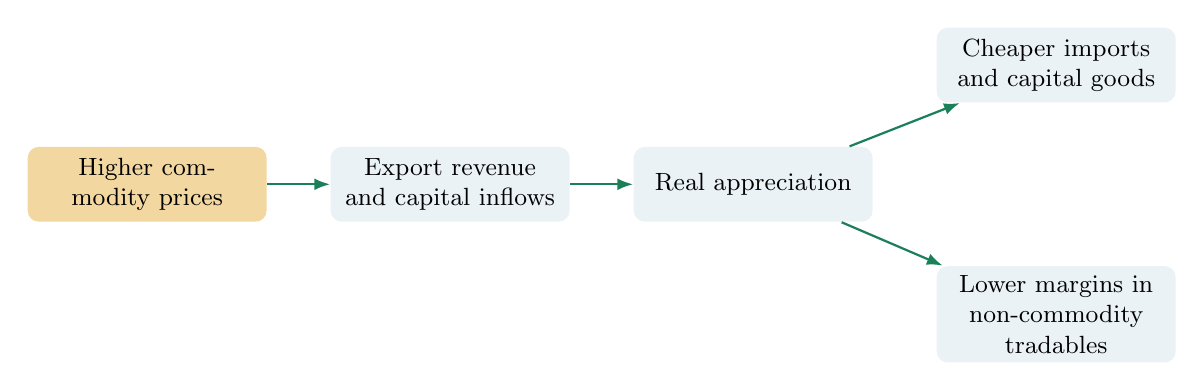
\begin{tikzpicture}[node distance=.55cm and .8cm,
    box/.style={rounded corners,minimum height=.95cm,text width=2.8cm,
                align=center,font=\small,fill=Sky},
    arr/.style={-{Latex[length=2mm]},thick,BrazilGreen}]
    \node[box,fill=WarmGold!45] (boom) {Higher commodity prices};
    \node[box,right=of boom] (flows) {Export revenue and capital inflows};
    \node[box,right=of flows] (app) {Real appreciation};
    \node[box,above right=of app] (gain) {Cheaper imports and capital goods};
    \node[box,below right=of app] (loss) {Lower margins in non-commodity tradables};
    \draw[arr] (boom)--(flows);
    \draw[arr] (flows)--(app);
    \draw[arr] (app)--(gain);
    \draw[arr] (app)--(loss);
  \end{tikzpicture}
  }
  \end{center}
  \vspace{.4cm}
  \begin{itemize}
    \item The exchange rate distributes a terms-of-trade shock across consumers and sectors.
    \item ``Dutch disease'' is a mechanism to test, not a complete diagnosis.
  \end{itemize}
\end{frame}

% 22
\begin{frame}{A weaker currency has ambiguous development effects}
  \scriptsize
  \begin{tabularx}{\textwidth}{>{\bfseries}p{2.6cm}XX}
    \toprule
    Margin & Possible gain from depreciation & Possible cost \\
    \midrule
    Exporters & Higher domestic-currency revenue & Imported inputs and financing become costlier \\
    Import-competing firms & More price space & Capital goods and technology cost more \\
    Households & Employment may shift toward tradables & Food, fuel, and durable goods become dearer \\
    Public sector & Some revenues rise with nominal activity & Indexed debt and inflation costs can increase \\
    Productivity & Entry into tradables may support learning & Protection can preserve low-productivity firms \\
    \bottomrule
  \end{tabularx}
  \vspace{.35cm}
  \question{The answer depends on balance sheets, imported-input intensity, credibility, and persistence.}
\end{frame}

% 23
\begin{frame}{Reserve accumulation changed Brazil's external buffer}
  \datagraphic{fig_reserves.pdf}
  \begin{itemize}
    \item Reserves insure against external funding stops and reduce foreign-currency liquidity risk.
    \item The stock rose sharply before the global financial crisis and has remained large.
  \end{itemize}
  \source{BCB SGS 13621. International reserves, cash concept; last daily observation of each month, US\$ billion.}
\end{frame}

% 26
\begin{frame}{The post-1999 framework combines adjustment and anchors}
  \begin{center}
  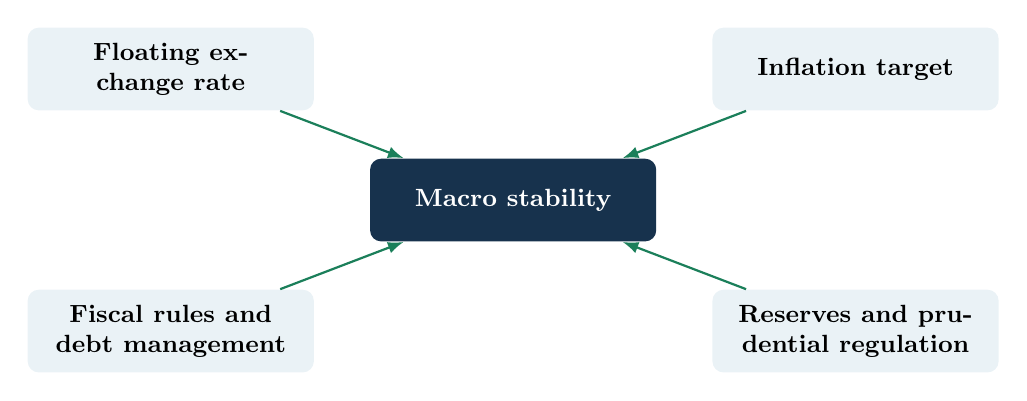
\begin{tikzpicture}[node distance=.6cm and .7cm,
    box/.style={rounded corners,minimum height=1.05cm,text width=3.4cm,
                align=center,font=\small\bfseries,fill=Sky},
    arr/.style={-{Latex[length=2mm]},thick,BrazilGreen}]
    \node[box,fill=DeepNavy,text=white] (core) {Macro stability};
    \node[box,above left=of core] (fx) {Floating exchange rate};
    \node[box,above right=of core] (it) {Inflation target};
    \node[box,below left=of core] (fisc) {Fiscal rules and debt management};
    \node[box,below right=of core] (buffer) {Reserves and prudential regulation};
    \draw[arr] (fx)--(core);
    \draw[arr] (it)--(core);
    \draw[arr] (fisc)--(core);
    \draw[arr] (buffer)--(core);
  \end{tikzpicture}
  \end{center}
  \vspace{.35cm}
  \begin{itemize}
    \item The pieces are complements: fiscal risk affects interest rates and the currency.
    \item The float absorbs shocks; monetary credibility limits pass-through.
  \end{itemize}
\end{frame}

% 27
\begin{frame}{Brazil's fiscal problem is about composition and credibility}
  \begin{columns}[T,onlytextwidth]
    \column{.48\textwidth}
      \begin{block}{The state is not small}
        Revenue and social spending are substantial for an upper-middle-income economy.
      \end{block}
      \vspace{.25cm}
      \begin{block}{Much spending is rigid}
        Pensions, payroll, transfers, and earmarks limit annual reallocation.
      \end{block}
    \column{.48\textwidth}
      \begin{exampleblock}{Development margin}
        Public investment and high-return maintenance compete for residual fiscal space.
      \end{exampleblock}
      \vspace{.25cm}
      \begin{exampleblock}{Macro margin}
        Uncertain debt paths raise risk premia and shorten private planning horizons.
      \end{exampleblock}
  \end{columns}
  \source{OECD, \href{https://www.oecd.org/en/publications/2023/12/oecd-economic-surveys-brazil-2023_7de8b505.html}{Economic Survey: Brazil 2023}.}
\end{frame}

\begin{frame}{Debt dynamics compress the space for development spending}
  \datagraphic{fig_gross_debt.pdf}
  \begin{itemize}
    \item Debt rose before the pandemic, jumped in 2020, and remains high relative to the mid-2000s.
    \item Interest rates, primary balances, growth, and debt composition jointly determine the path.
  \end{itemize}
  \source{BCB SGS 13762. Gross general government debt, methodology used since 2008, monthly, percent of GDP.}
\end{frame}

% 28
\begin{frame}{Low saving and investment constrain capital deepening}
  \begin{columns}[T,onlytextwidth]
    \column{.44\textwidth}
      \begin{center}
        {\fontsize{34}{38}\selectfont\color{DeepNavy}\textbf{16.8\%}}\\[-.1cm]
        \muted{investment / GDP, 2025}
        \vspace{.7cm}

        {\fontsize{34}{38}\selectfont\color{BrazilGreen}\textbf{14.4\%}}\\[-.1cm]
        \muted{saving / GDP, 2025}
      \end{center}
    \column{.52\textwidth}
      \begin{itemize}
        \item Capital per worker grows slowly when investment remains low.
        \item High financing costs screen out long-horizon projects.
        \item Infrastructure bottlenecks reduce the return to private capital.
        \item Productivity growth matters because more investment alone can misallocate resources.
      \end{itemize}
  \end{columns}
  \source{IBGE, National Accounts 2025; rates are shares of GDP.}
\end{frame}

% 29
\begin{frame}{Macro scorecard: a major achievement and an incomplete transition}
  \scriptsize
  \begin{tabularx}{\textwidth}{>{\bfseries}p{2.4cm}XX}
    \toprule
    Area & Achievement & Remaining constraint \\
    \midrule
    Inflation & Hyperinflation ended; expectations have an explicit anchor & Shocks still pass through the currency and indexation \\
    Exchange rate & A float absorbs external shocks & Volatility affects prices, balance sheets, and investment \\
    External sector & Reserves and lower FX mismatch strengthened buffers & Commodity and global-rate cycles remain important \\
    Fiscal policy & Strong revenue capacity and broad social insurance & Rigid spending and debt uncertainty compress investment \\
    Capital formation & Deep domestic financial markets & High cost of capital and low investment \\
    \bottomrule
  \end{tabularx}
\end{frame}

% 30
\begin{frame}[plain]
  \begin{tikzpicture}[remember picture,overlay]
    \fill[WarmGray] (current page.south west) rectangle (current page.north east);
    \node[text=DeepNavy,font=\bfseries\fontsize{30}{34}\selectfont] at (current page.center)
      {10-minute break};
    \node[text=MidGray,font=\large,below=.55cm of current page.center]
      {After the break: why stability did not restore convergence};
  \end{tikzpicture}
\end{frame}

% 31
\sectionframe{Part II -- Making growth happen}{Productivity, firms, workers, and the institutions that connect them}

% 32
\begin{frame}{Stability raises the return to investment; it does not guarantee it}
  \begin{center}
  \resizebox{.94\textwidth}{!}{%
  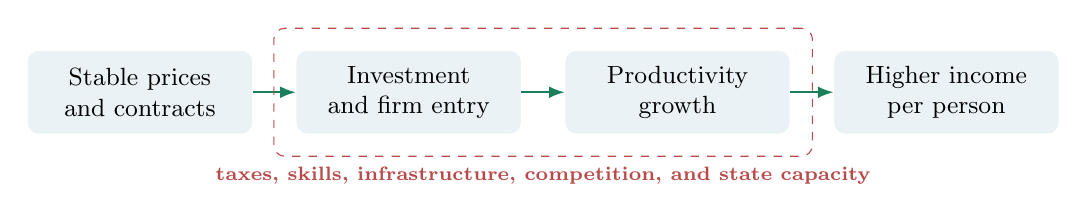
\begin{tikzpicture}[node distance=.55cm,
    box/.style={rounded corners,minimum width=2.85cm,minimum height=1.05cm,
                text width=2.55cm,align=center,font=\small,fill=Sky},
    arr/.style={-{Latex[length=2mm]},thick,BrazilGreen}]
    \node[box] (stable) {Stable prices and contracts};
    \node[box,right=of stable] (invest) {Investment and firm entry};
    \node[box,right=of invest] (prod) {Productivity growth};
    \node[box,right=of prod] (income) {Higher income per person};
    \draw[arr] (stable)--(invest);
    \draw[arr] (invest)--(prod);
    \draw[arr] (prod)--(income);
    \node[draw=Brick,dashed,rounded corners,fit=(invest)(prod),inner sep=8pt,
          label={[text=Brick,font=\scriptsize\bfseries]below:taxes, skills, infrastructure, competition, and state capacity}] {};
  \end{tikzpicture}
  }
  \end{center}
  \vspace{.75cm}
  \question{Brazil solved much of the first arrow. The middle of the chain remains weak.}
\end{frame}

% 33
\begin{frame}{Aggregate productivity depends on firms and allocation}
  \[
    \text{Aggregate productivity}
    = \underbrace{\text{productivity within firms}}_{\substack{\text{technology, management,}\\\text{skills, scale}}}
    + \underbrace{\text{allocation across firms}}_{\substack{\text{entry, exit, competition,}\\\text{capital and labor flows}}}
  \]
  \vspace{.45cm}
  \begin{columns}[T,onlytextwidth]
    \column{.48\textwidth}
      \begin{block}{Within-firm margin}
        Can an existing producer adopt better technology and organization?
      \end{block}
    \column{.48\textwidth}
      \begin{exampleblock}{Reallocation margin}
        Do productive firms expand while persistently unproductive firms shrink or exit?
      \end{exampleblock}
  \end{columns}
\end{frame}

% 34
\begin{frame}{Brazil's productivity problem is not uniform across sectors}
  \datagraphic{fig_sector_productivity.pdf}
  \begin{itemize}
    \item Agriculture shows that sustained productivity growth is possible.
    \item Services employ most workers, so diffusion beyond the frontier sector determines the aggregate result.
  \end{itemize}
  \source{World Bank, labor-productivity growth by sector, 1996--2020; values rounded.}
\end{frame}

% 35
\begin{frame}{A long tail of low-productivity firms shapes aggregate outcomes}
  \begin{columns}[T,onlytextwidth]
    \column{.47\textwidth}
      \begin{block}{The long tail}
        Many small producers use little capital, management technology, or formal finance.
      \end{block}
      \vspace{.3cm}
      \begin{exampleblock}{The frontier}
        A smaller set of firms competes globally and adopts advanced technology.
      \end{exampleblock}
    \column{.49\textwidth}
      \begin{itemize}
        \item Informality lowers tax and regulatory costs but limits scale and credit access.
        \item Complex rules encourage firms to remain small or split activities.
        \item Weak exit and reallocation preserve low-productivity uses of capital and labor.
      \end{itemize}
  \end{columns}
\end{frame}

\begin{frame}{Firm capabilities determine whether technology is adopted}
  \begin{columns}[T,onlytextwidth]
    \column{.31\textwidth}
      \begin{block}{Management}
        Targets, inventory control, quality systems, and worker incentives.
      \end{block}
    \column{.31\textwidth}
      \begin{block}{Technology}
        Digital tools pay off only when processes and skills change with them.
      \end{block}
    \column{.31\textwidth}
      \begin{block}{Scale}
        Formal finance and access to larger markets allow fixed costs to be spread.
      \end{block}
  \end{columns}
  \vspace{.7cm}
  \question{Credit subsidies alone do little when management, competition, and demand remain unchanged.}
  \source{World Bank, Brazil productivity diagnostics; OECD, Economic Survey: Brazil 2023.}
\end{frame}

\begin{frame}{Informality is both insurance and a productivity trap}
  \begin{columns}[T,onlytextwidth]
    \column{.48\textwidth}
      \begin{block}{Why workers and firms enter}
        Low entry costs, flexible hours, weak formal-job creation, and immediate income.
      \end{block}
      \vspace{.25cm}
      \begin{block}{What it provides}
        A margin of adjustment when formal employment and social insurance do not reach everyone.
      \end{block}
    \column{.48\textwidth}
      \begin{exampleblock}{What it limits}
        Credit, training, scale, legal enforcement, tax capacity, and portable protection.
      \end{exampleblock}
      \vspace{.25cm}
      \begin{exampleblock}{Policy margin}
        Lower formalization cliffs and make benefits portable across employment types.
      \end{exampleblock}
  \end{columns}
  \source{IBGE, PNAD Continua; OECD, Economic Survey: Brazil 2023. Informality is a statistical labor-market category, not a synonym for tax evasion.}
\end{frame}

% 36
\begin{frame}{Embrapa shows how complementary institutions raise productivity}
  \begin{center}
  
\begin{tikzpicture}[node distance=.42cm,
    box/.style={rounded corners,minimum height=1.0cm,text width=2.55cm,
                align=center,font=\scriptsize,fill=Sky},
    arr/.style={-{Latex[length=1.8mm]},thick,BrazilGreen}]
    \node[box,fill=DeepNavy,text=white] (research) {Public agricultural research};
    \node[box,right=of research] (tech) {Soil correction, seeds, and tropical techniques};
    \node[box,right=of tech] (diff) {Extension, credit, logistics, and diffusion};
    \node[box,right=of diff,fill=WarmGold!40] (prod) {Private investment and productivity};
    \draw[arr] (research)--(tech);
    \draw[arr] (tech)--(diff);
    \draw[arr] (diff)--(prod);
  \end{tikzpicture}
  \end{center}
  \vspace{.55cm}
  \begin{columns}[T,onlytextwidth]
    \column{.48\textwidth}
      \begin{block}{Lesson}
        Mission-oriented research works when adoption, finance, and infrastructure reinforce it.
      \end{block}
    \column{.48\textwidth}
      \begin{exampleblock}{Trade-off}
        Productivity per hectare and environmental enforcement jointly determine land-use outcomes.
      \end{exampleblock}
  \end{columns}
  \source{Embrapa Cerrados; Ipea, agricultural productivity.}
\end{frame}

% 37
\begin{frame}{``Custo Brasil'' is a system of interacting wedges}
  \begin{center}
  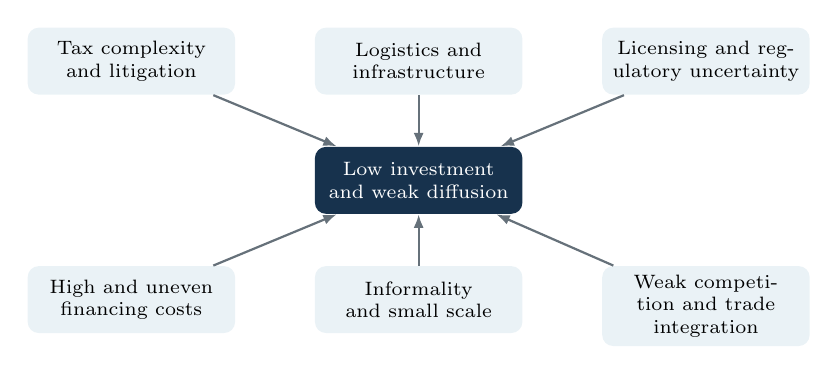
\begin{tikzpicture}[node distance=.65cm and 1.0cm,
    box/.style={rounded corners,minimum height=.85cm,text width=2.4cm,
                align=center,font=\scriptsize,fill=Sky},
    arr/.style={-{Latex[length=1.7mm]},thick,MidGray}]
    \node[box,fill=DeepNavy,text=white] (core) {Low investment and weak diffusion};
    \node[box,above left=of core] (tax) {Tax complexity and litigation};
    \node[box,above=of core] (infra) {Logistics and infrastructure};
    \node[box,above right=of core] (reg) {Licensing and regulatory uncertainty};
    \node[box,below left=of core] (credit) {High and uneven financing costs};
    \node[box,below=of core] (informal) {Informality and small scale};
    \node[box,below right=of core] (comp) {Weak competition and trade integration};
    \foreach \n in {tax,infra,reg,credit,informal,comp}{\draw[arr] (\n)--(core);}
  \end{tikzpicture}
  \end{center}
  \vspace{.25cm}
  \question{Removing one wedge may have little effect when the other complements remain binding.}
\end{frame}

% 38
\begin{frame}{The consumption-tax reform is a live implementation test}
  \begin{columns}[T,onlytextwidth]
    \column{.23\textwidth}\begin{block}{2026}Test year for CBS and IBS.\end{block}
    \column{.23\textwidth}\begin{block}{2027}CBS begins; PIS/Cofins end.\end{block}
    \column{.23\textwidth}\begin{block}{2029--32}Gradual ICMS/ISS transition.\end{block}
    \column{.23\textwidth}\begin{block}{2033}Full new system.\end{block}
  \end{columns}
  \vspace{.45cm}
  \begin{itemize}
    \item A destination-based VAT should reduce cascading taxes and production distortions.
    \item Federal coordination, exemptions, compliance systems, and transition rules determine the gain.
    \item Implementation is an economic reform, not an administrative footnote.
  \end{itemize}
  \source{Receita Federal, \href{https://www.gov.br/receitafederal/pt-br/acesso-a-informacao/acoes-e-programas/programas-e-atividades/reforma-tributaria-do-consumo/entenda}{Consumption Tax Reform}.}
\end{frame}

\begin{frame}{Competition policy changes the return to innovation}
  \begin{columns}[T,onlytextwidth]
    \column{.47\textwidth}
      \begin{block}{When entry is credible}
        Incumbents invest, lower markups, and adopt technology to defend market share.
      \end{block}
    \column{.49\textwidth}
      \begin{exampleblock}{When rents are protected}
        Licensing, procurement design, network bottlenecks, and local political connections can preserve inefficient firms.
      \end{exampleblock}
  \end{columns}
  \vspace{.6cm}
  \begin{itemize}
    \item Antitrust, bankruptcy, trade exposure, and transparent procurement affect the same reallocation margin.
    \item The objective is contestability, not a mechanical preference for large or small firms.
  \end{itemize}
  \source{OECD, Competition Assessment Reviews: Brazil; CADE, institutional reports.}
\end{frame}

\begin{frame}{Logistics determine which firms can reach national markets}
  \begin{columns}[T,onlytextwidth]
    \column{.31\textwidth}\begin{block}{Distance}A continental economy makes transport time and reliability part of marginal cost.\end{block}
    \column{.31\textwidth}\begin{block}{Networks}Roads, rail, ports, storage, and digital systems are complements.\end{block}
    \column{.31\textwidth}\begin{block}{Governance}Project selection, maintenance, concessions, and licensing determine returns.\end{block}
  \end{columns}
  \vspace{.65cm}
  \question{A new asset raises productivity only if the network around it works.}
  \source{World Bank, Brazil infrastructure diagnostics; EPL/Infra S.A., National Logistics Plan.}
\end{frame}

\begin{frame}{Sanitation is infrastructure and human-capital policy}
  \begin{columns}[T,onlytextwidth]
    \column{.48\textwidth}
      \begin{block}{Household channel}
        Water quality and sewage coverage affect disease, school attendance, time use, and property values.
      \end{block}
    \column{.48\textwidth}
      \begin{exampleblock}{Implementation channel}
        Municipal scale, regulation, contracts, and service affordability shape expansion.
      \end{exampleblock}
  \end{columns}
  \vspace{.65cm}
  \begin{itemize}
    \item National averages conceal large regional and within-city gaps.
    \item Universalization requires investment and credible regulation, not construction alone.
  \end{itemize}
  \source{SNIS, Ministry of Cities; IBGE, 2022 Population Census sanitation results.}
\end{frame}

% 39
\begin{frame}{Trade can raise productivity through inputs, scale, and selection}
  \begin{columns}[T,onlytextwidth]
    \column{.47\textwidth}
      \begin{block}{Channels}
        \begin{itemize}
          \item Cheaper and better intermediate inputs
          \item Larger markets for productive exporters
          \item Technology and management diffusion
          \item Entry and exit under competition
        \end{itemize}
      \end{block}
    \column{.49\textwidth}
      \begin{exampleblock}{Transition costs}
        \begin{itemize}
          \item Workers and places adjust slowly
          \item Logistics and customs can bind first
          \item A volatile real exchange rate changes incentives
          \item Skills determine who captures the gains
        \end{itemize}
      \end{exampleblock}
  \end{columns}
  \vspace{.35cm}
  \question{The relevant choice is the sequence and support for adjustment, not autarky versus free trade.}
\end{frame}

\begin{frame}{The credit spread remains a microeconomic wedge}
  \datagraphic{fig_credit_spread.pdf}
  \begin{itemize}
    \item The spread combines expected losses, operating costs, taxes, market power, and risk premia.
    \item Better collateral, information sharing, competition, and insolvency rules address different components.
  \end{itemize}
  \source{BCB SGS 20783. Average spread on outstanding credit, monthly, percentage points.}
\end{frame}

% 40
\begin{frame}{The human-capital constraint is learning, not enrollment alone}
  \datagraphic{fig_pisa_math.pdf}
  \begin{itemize}
    \item Learning gaps reduce adoption of technology and worker mobility.
    \item Teacher practice, early childhood, completion, and school governance operate at different horizons.
  \end{itemize}
  \source{OECD, \href{https://www.oecd.org/en/publications/pisa-2022-results-volume-i-and-ii-country-notes_ed6fbcc5-en/brazil_61690648-en.html}{PISA 2022: Brazil}.}
\end{frame}

\begin{frame}{Human capital starts before school and differs by place}
  \begin{columns}[T,onlytextwidth]
    \column{.31\textwidth}\begin{block}{Early childhood}Nutrition, health, language exposure, and childcare shape readiness.\end{block}
    \column{.31\textwidth}\begin{block}{School system}Teacher support and instructional time determine whether enrollment becomes learning.\end{block}
    \column{.31\textwidth}\begin{block}{Territory}Transport, violence, sanitation, and local fiscal capacity affect access and continuity.\end{block}
  \end{columns}
  \vspace{.65cm}
  \question{Equal spending does not imply equal learning when local constraints differ.}
  \source{World Bank, Brazil Human Capital Review; IBGE and Inep education indicators.}
\end{frame}

% 41
\begin{frame}{Low unemployment can coexist with a dual labor market}
  \begin{columns}[T,onlytextwidth]
    \column{.72\textwidth}
      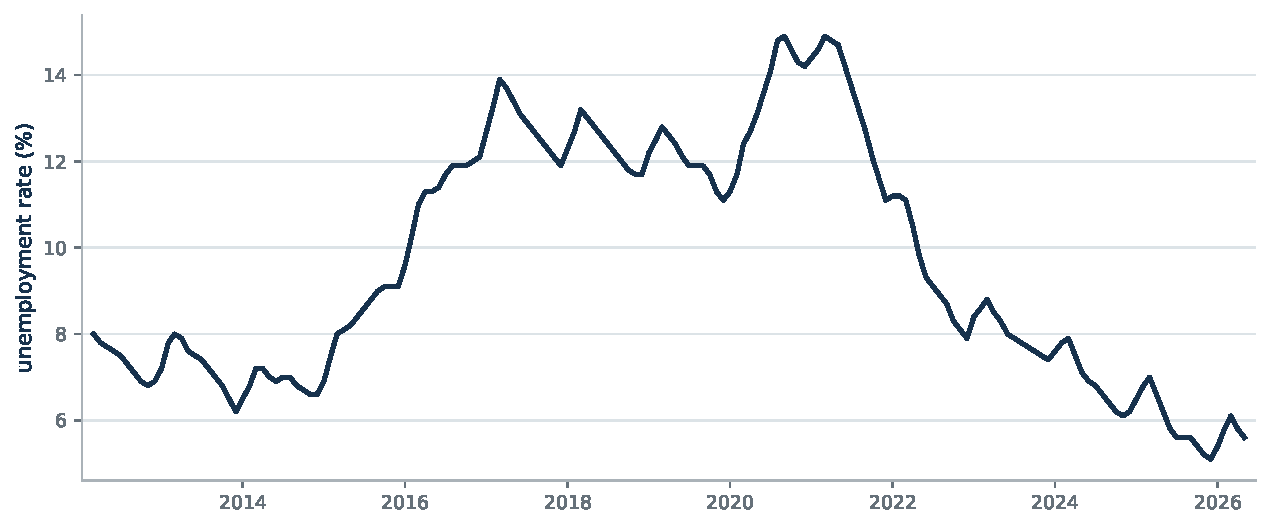
\includegraphics[width=\linewidth,height=.58\textheight,keepaspectratio]{fig_unemployment.pdf}
    \column{.25\textwidth}
      \begin{block}{Informality}
        \centering
        {\fontsize{27}{30}\selectfont\color{Brick}\textbf{38.1\%}}\\
        of workers in 2025
      \end{block}
      \begin{itemize}\scriptsize
        \item flexibility and income
        \item weak insurance and training
        \item lower firm scale
      \end{itemize}
  \end{columns}
  \source{BCB SGS 24369, sourced from IBGE PNAD Continua; IBGE annual informality rate for 2025.}
\end{frame}

\begin{frame}{Childcare expands labor supply and children's capabilities}
  \begin{columns}[T,onlytextwidth]
    \column{.48\textwidth}
      \begin{block}{Labor-market effect}
        Affordable, reliable childcare raises mothers' ability to take formal jobs and invest in careers.
      \end{block}
    \column{.48\textwidth}
      \begin{exampleblock}{Human-capital effect}
        Quality matters: childcare can improve language, nutrition, and school readiness.
      \end{exampleblock}
  \end{columns}
  \vspace{.7cm}
  \begin{itemize}
    \item Coverage, hours, location, and quality jointly determine take-up.
    \item The return is highest when expansion targets families with the largest access gaps.
  \end{itemize}
  \source{IBGE, PNAD Continua care responsibilities; World Bank, Brazil gender and human-capital diagnostics.}
\end{frame}

% 42
\begin{frame}{Growth and redistribution are not opposing mechanisms}
  \begin{center}
  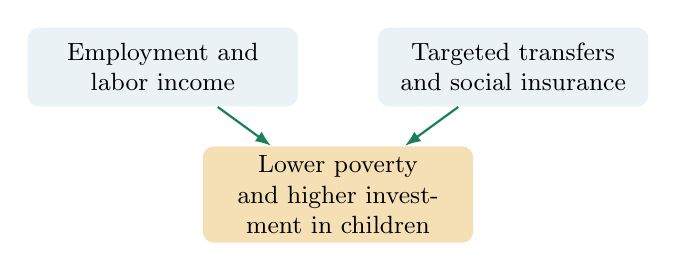
\begin{tikzpicture}[node distance=.7cm and 1.0cm,
    box/.style={rounded corners,minimum height=1.0cm,text width=3.2cm,
                align=center,font=\small,fill=Sky},
    arr/.style={-{Latex[length=2mm]},thick,BrazilGreen}]
    \node[box] (jobs) {Employment and labor income};
    \node[box,right=of jobs] (transfers) {Targeted transfers and social insurance};
    \node[box,below=1.0cm of $(jobs)!0.5!(transfers)$,fill=WarmGold!35] (poverty)
      {Lower poverty and higher investment in children};
    \draw[arr] (jobs)--(poverty);
    \draw[arr] (transfers)--(poverty);
  \end{tikzpicture}
  \end{center}
  \vspace{.4cm}
  \begin{itemize}
    \item Recent poverty reduction reflects both labor income and transfers.
    \item Benefit design should preserve coverage while reducing abrupt formalization penalties.
    \item Poverty rates must always report the line and purchasing-power standard used.
  \end{itemize}
  \source{Ipea, Poverty and Inequality, 1995--2024; IBGE, Social Indicators 2025.}
\end{frame}

% 43
\begin{frame}{Pix is a case of digital public infrastructure}
  \begin{columns}[T,onlytextwidth]
    \column{.44\textwidth}
      \begin{center}
        {\fontsize{32}{36}\selectfont\color{DeepNavy}\textbf{170m+}}\\[-.1cm]
        \muted{individual users}
        \vspace{.55cm}

        {\fontsize{32}{36}\selectfont\color{BrazilGreen}\textbf{7bn+}}\\[-.1cm]
        \muted{transactions in January 2026}
      \end{center}
    \column{.52\textwidth}
      \begin{itemize}
        \item The central bank set common rails, rules, and access standards.
        \item Private institutions compete on top of a public protocol.
        \item Immediate settlement lowers payment frictions for households and small firms.
        \item Fraud, digital access, and over-indebtedness remain policy concerns.
      \end{itemize}
  \end{columns}
  \source{BCB, \href{https://www.bcb.gov.br/estabilidadefinanceira/estatisticaspix}{Pix Statistics}; figures reported in early 2026.}
\end{frame}

\begin{frame}{Spatial inequality changes which reform binds first}
  \begin{columns}[T,onlytextwidth]
    \column{.31\textwidth}\begin{block}{Productive structure}Agriculture, industry, services, and public employment have different regional weights.\end{block}
    \column{.31\textwidth}\begin{block}{Local capacity}Municipalities differ in tax bases, technical staff, procurement, and service networks.\end{block}
    \column{.31\textwidth}\begin{block}{Household access}Transport, schools, health, sanitation, and security shape mobility within the same city.\end{block}
  \end{columns}
  \vspace{.65cm}
  \question{A national reform produces local results through unequal implementation capacity.}
  \source{IBGE, Regional Accounts and 2022 Population Census; Ipea, regional development studies.}
\end{frame}

\begin{frame}{State capacity is an economic input}
  \begin{columns}[T,onlytextwidth]
    \column{.48\textwidth}
      \begin{block}{Administrative capacity}
        Select projects, hire staff, procure inputs, manage contracts, and use data.
      \end{block}
      \vspace{.25cm}
      \begin{block}{Legal capacity}
        Enforce contracts, protect rights, resolve disputes, and sanction corruption.
      \end{block}
    \column{.48\textwidth}
      \begin{exampleblock}{Fiscal capacity}
        Raise revenue with low compliance costs and allocate it toward high-return services.
      \end{exampleblock}
      \vspace{.25cm}
      \begin{exampleblock}{Coordination capacity}
        Align federal, state, and municipal responsibilities across shared networks.
      \end{exampleblock}
  \end{columns}
  \source{World Bank, The Brazil of the Future; OECD, Government at a Glance: Latin America and the Caribbean.}
\end{frame}

\sectionframe{Micro lens -- Security and development}{How coercive territorial power changes markets, services, and state capacity}

\begin{frame}{Organized crime is a microeconomic constraint}
  \begin{center}
  \resizebox{.94\textwidth}{!}{%
  
\begin{tikzpicture}[node distance=.45cm,
    box/.style={rounded corners,minimum height=1.05cm,text width=3.0cm,align=center,font=\small,fill=Sky},
    arr/.style={-{Latex[length=2mm]},thick,BrazilGreen}]
    \node[box,fill=DeepNavy,text=white] (power) {Coercive territorial power};
    \node[box,right=of power] (wedges) {Illegal taxation, entry barriers, and capture};
    \node[box,right=of wedges] (markets) {Weaker competition and public services};
    \node[box,right=of markets,fill=WarmGold!35] (outcomes) {Lower investment, mobility, and human capital};
    \draw[arr] (power)--(wedges); \draw[arr] (wedges)--(markets); \draw[arr] (markets)--(outcomes);
  \end{tikzpicture}}
  \end{center}
  \vspace{.55cm}
  \begin{itemize}
    \item Extortion acts like an illegal tax; forced suppliers create local market power.
    \item Land appropriation weakens property rights and collateral.
    \item Intimidation and corruption can redirect enforcement and public resources.
  \end{itemize}
  \source{MPRJ documented cases; SENAPPEN; GENI/UFF and Instituto Fogo Cruzado. Mechanisms are not estimates of aggregate GDP losses.}
\end{frame}

\begin{frame}{There is no single organized-crime statistic}
  \begin{columns}[T,onlytextwidth]
    \column{.31\textwidth}
      \begin{block}{Lethal violence}
        \textbf{Unit:} deaths\\[.15cm]
        National and annual. It does not identify the organization responsible.
      \end{block}
    \column{.31\textwidth}
      \begin{block}{Prison intelligence}
        \textbf{Unit:} groups\\[.15cm]
        SENAPPEN identified at least 88 organizations affecting prisons in its 2024 exercise.
      \end{block}
    \column{.31\textwidth}
      \begin{block}{Territorial control}
        \textbf{Unit:} places and residents\\[.15cm]
        Directly measures armed governance, but only for Metropolitan Rio.
      \end{block}
  \end{columns}
  \vspace{.6cm}
  \question{Measurement must match the mechanism being discussed.}
  \source{Ipea/FBSP, Atlas da Violencia 2026; SENAPPEN, Mapa das ORCRIMs; GENI/UFF and Instituto Fogo Cruzado, 2025.}
\end{frame}

\begin{frame}{Lethal violence fell, but data quality changes the trend}
  \datagraphic{fig_homicide_rates.pdf}
  \begin{itemize}
    \item The registered rate fell after 2017; reallocating some deaths of undetermined cause produces a smaller decline.
    \item Homicide measures lethal violence. It does not measure the size or revenue of criminal organizations.
  \end{itemize}
  \source{Ipea and FBSP, Atlas da Violencia 2026, based on SIM/Ministry of Health and IBGE. Rates per 100,000. Estimated series is model-based.}
\end{frame}

\begin{frame}{Metropolitan Rio shows the scale of territorial armed governance}
  \datagraphic{fig_rio_territorial_control.pdf}
  \begin{itemize}
    \item In 2024, 34.9\% of residents were estimated to live under armed-group control or influence.
    \item The estimate covers Metropolitan Rio, uses anonymous reporting, and is not a national census.
  \end{itemize}
  \source{GENI/UFF and Instituto Fogo Cruzado, Mapa Historico dos Grupos Armados 2025, with 2022 Census population data. Published shares are rounded.}
\end{frame}

\begin{frame}{Coercive market power reaches ordinary goods and services}
  \begin{columns}[T,onlytextwidth]
    \column{.31\textwidth}
      \begin{block}{Household services}
        Cooking gas, broadband, cable TV, and electricity.
      \end{block}
      \begin{block}{Mobility}
        Alternative transport and compulsory payments from drivers.
      \end{block}
    \column{.31\textwidth}
      \begin{block}{Property}
        Irregular construction, forced dispossession, and property sales.
      \end{block}
      \begin{block}{Local retail}
        Security fees, merchant extortion, and forced suppliers.
      \end{block}
    \column{.31\textwidth}
      \begin{exampleblock}{Economic wedges}
        \begin{itemize}\scriptsize
          \item illegal tax
          \item restricted entry
          \item weak property rights
          \item distorted procurement
        \end{itemize}
      \end{exampleblock}
  \end{columns}
  \source{MPRJ cases in Nova Iguacu (2019), Itaborai (2019), Queimados (2024), and the illegal-construction task force (2022). These cases do not measure national prevalence.}
\end{frame}

\begin{frame}{Territorial violence erodes human capital}
  \begin{columns}[T,onlytextwidth]
    \column{.31\textwidth}
      \begin{block}{Exposure}
        \centering{\fontsize{27}{30}\selectfont\color{Brick}\textbf{51\%}}\\
        of students in the 19 municipalities studied were affected by armed violence in 2022.
      \end{block}
    \column{.31\textwidth}
      \begin{block}{Learning}
        \centering{\fontsize{27}{30}\selectfont\color{DeepNavy}\textbf{10 points}}\\
        maximum reported SAEB gap, interpreted by the authors as about six months of learning.
      \end{block}
    \column{.31\textwidth}
      \begin{block}{Dropout}
        \centering{\fontsize{24}{27}\selectfont\color{BrazilGreen}\textbf{7.2 vs. 9.0--9.6\%}}\\
        non-controlled versus controlled areas in Metropolitan Rio.
      \end{block}
  \end{columns}
  \vspace{.35cm}
  \source{UNICEF, Educacao Sob Cerco 2025, with GENI/UFF and Instituto Fogo Cruzado. Conditional estimates with statistical controls; the design is not experimental.}
\end{frame}

\begin{frame}{A credible response combines enforcement and service delivery}
  \scriptsize
  \begin{tabularx}{\textwidth}{>{\bfseries}p{2.35cm}XX}
    \toprule
    Margin & Instruments & Development outcome \\
    \midrule
    Territorial prevention & Safe routes, reliable transport, service continuity, youth prevention & Attendance, business entry, service uptime \\
    Investigation and justice & Forensics, witness protection, case management, corruption control & Clearance with due process, time to disposition \\
    Financial disruption & Beneficial ownership, intelligence, freezing and confiscation & Assets finally recovered, disrupted cash flow \\
    Sector regulation & Internet, fuels, fintech, construction, health, procurement & Prices, entry, ownership transparency \\
    Prison governance & Intelligence, lawful communications control, work and reintegration & Violence, illicit communication, recidivism \\
    \bottomrule
  \end{tabularx}
  \source{MJSP, ENFOC and ENCCLA; SENAPPEN/CNPCP, National Criminal and Penitentiary Policy Plan 2024--2027.}
\end{frame}

\begin{frame}{Discussion: what outcome would demonstrate greater state capacity?}
  \vspace{.2cm}
  \question{Choose one instrument and the final outcome that should be used to evaluate it.}
  \vspace{.55cm}
  \begin{columns}[T,onlytextwidth]
    \column{.23\textwidth}\begin{block}{Operations}Activity measure\end{block}
    \column{.23\textwidth}\begin{block}{Arrests}Intermediate output\end{block}
    \column{.23\textwidth}\begin{block}{Recovered assets}Financial outcome\end{block}
    \column{.23\textwidth}\begin{block}{Market entry}Development outcome\end{block}
  \end{columns}
  \vspace{.55cm}
  \begin{itemize}
    \item Add one safeguard against abuse or displacement to another territory.
    \item Explain why your chosen outcome is closer to welfare than the activity count.
  \end{itemize}
\end{frame}

% 44
\begin{frame}{Micro scorecard: strong examples, weak diffusion}
  \scriptsize
  \begin{tabularx}{\textwidth}{>{\bfseries}p{2.25cm}XX}
    \toprule
    Area & Evidence of capability & Binding margin \\
    \midrule
    Technology & Agricultural research and digital finance & Diffusion beyond frontier sectors \\
    Firms & Globally competitive exporters and banks & Long tail of small, informal producers \\
    Tax system & Reform establishes a modern VAT structure & Transition, exemptions, and implementation \\
    Trade & Competitive commodity and selected manufacturing exports & Low integration and costly inputs \\
    Workers & Broad enrollment and recent labor-market strength & Learning gaps and informality \\
    Infrastructure & Scalable concessions and digital public rails & Logistics, sanitation, and local coordination \\
    State capacity & Strong agencies and data systems in selected areas & Uneven local capacity and territorial coercion \\
    \bottomrule
  \end{tabularx}
\end{frame}

\begin{frame}{Demography raises the return to productivity now}
  \datagraphic{fig_ageing.pdf}
  \begin{itemize}
    \item The working-age share will no longer provide the same contribution to growth.
    \item Health, pensions, care, lifelong learning, and later-life employment become linked policies.
  \end{itemize}
  \source{IBGE, Population Projections 2024. The 2070 value is a projection, not an observed outcome.}
\end{frame}

% 45
\begin{frame}{Three clocks tighten the development constraint}
  \begin{columns}[T,onlytextwidth]
    \column{.31\textwidth}
      \begin{block}{Demography}
        Population peaks around 2041. The 60+ share rises from 15.6\% in 2023 to 37.8\% in 2070.
      \end{block}
    \column{.31\textwidth}
      \begin{block}{Climate}
        Droughts, floods, heat, and land-use pressure affect capital, food, energy, and cities.
      \end{block}
    \column{.31\textwidth}
      \begin{block}{Fiscal space}
        Aging raises health and pension pressure while adaptation and infrastructure require investment.
      \end{block}
  \end{columns}
  \vspace{.7cm}
  \question{Future growth must rely more on productivity because labor-force expansion is ending.}
  \source{IBGE, Population Projections 2024; OECD, Economic Survey Brazil 2023.}
\end{frame}

% 46
\begin{frame}{Brazil has a green advantage and a territorial emissions problem}
  \begin{columns}[T,onlytextwidth]
    \column{.48\textwidth}
      \begin{exampleblock}{Energy advantage}
        \centering
        {\fontsize{34}{38}\selectfont\color{BrazilGreen}\textbf{86.6\%}}\\
        renewable domestic electricity supply in 2025
      \end{exampleblock}
      \begin{itemize}
        \item Hydro, wind, solar, biomass, and biofuels create options for low-carbon production.
      \end{itemize}
    \column{.48\textwidth}
      \begin{block}{Emissions structure}
        \centering
        {\fontsize{28}{32}\selectfont\color{Brick}\textbf{about 70\%}}\\
        from land use and agriculture in the 2022 inventory
      \end{block}
      \begin{itemize}
        \item Enforcement, livestock productivity, restoration, and urban adaptation are central.
      \end{itemize}
  \end{columns}
  \source{EPE, BEN 2026; MCTI, National Emissions Inventory, 2022 results.}
\end{frame}

% 47
\begin{frame}{The agenda is a package of complements}
  \begin{center}
  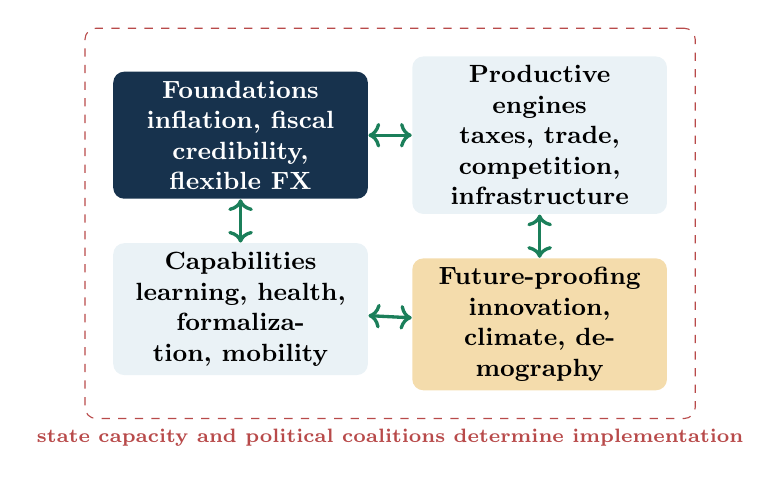
\begin{tikzpicture}[node distance=.55cm and .55cm,
    box/.style={rounded corners,minimum height=1.25cm,text width=3.0cm,
                align=center,font=\small\bfseries,fill=Sky}]
    \node[box,fill=DeepNavy,text=white] (found) {Foundations\\inflation, fiscal credibility, flexible FX};
    \node[box,right=of found] (eng) {Productive engines\\taxes, trade, competition, infrastructure};
    \node[box,below=of found] (cap) {Capabilities\\learning, health, formalization, mobility};
    \node[box,below=of eng,fill=WarmGold!40] (future) {Future-proofing\\innovation, climate, demography};
    \draw[very thick,BrazilGreen,<->] (found)--(eng);
    \draw[very thick,BrazilGreen,<->] (found)--(cap);
    \draw[very thick,BrazilGreen,<->] (eng)--(future);
    \draw[very thick,BrazilGreen,<->] (cap)--(future);
    \node[draw=Brick,dashed,rounded corners,fit=(found)(eng)(cap)(future),inner sep=10pt,
      label={[text=Brick,font=\scriptsize\bfseries]below:state capacity and political coalitions determine implementation}] {};
  \end{tikzpicture}
  \end{center}
\end{frame}

% 48
\begin{frame}{Priority exercise: allocate a reform budget}
  \vspace{.2cm}
  \question{Your group has R\$100 of political capital. Allocate it across the four pillars.}
  \vspace{.55cm}
  \begin{columns}[T,onlytextwidth]
    \column{.23\textwidth}
      \begin{block}{Foundations}
        R\$\rule{1.0cm}{.3pt}
      \end{block}
    \column{.23\textwidth}
      \begin{block}{Productive engines}
        R\$\rule{1.0cm}{.3pt}
      \end{block}
    \column{.23\textwidth}
      \begin{block}{Capabilities}
        R\$\rule{1.0cm}{.3pt}
      \end{block}
    \column{.23\textwidth}
      \begin{block}{Future-proofing}
        R\$\rule{1.0cm}{.3pt}
      \end{block}
  \end{columns}
  \vspace{.55cm}
  \begin{itemize}
    \item Name one complement without which your largest allocation would fail.
    \item Name one group or region that bears the transition cost.
  \end{itemize}
\end{frame}

% 49
\begin{frame}{The diagnosis is complementarity, not a single missing reform}
  \small
  \begin{itemize}
    \setlength\itemsep{.18cm}
    \item Macroeconomic stability protects planning horizons and keeps exchange-rate shocks from becoming persistent inflation.
    \item A flexible exchange rate, credible fiscal policy, and external buffers improve shock absorption.
    \item Productivity requires firms to adopt better methods and resources to move toward productive uses.
    \item State capacity protects rights, regulates markets, delivers services, and confronts territorial coercion.
    \item Inclusion, demography, and climate affect both the returns to reform and the coalition that can sustain it.
  \end{itemize}
  \vspace{.25cm}
  \question{Questions and discussion}
\end{frame}

\end{document}
